\subsection{Photometric correction}
\label{se:photometric_correction}

The \emph{baseline} calibration (Sect.~\ref{se:baseline_calibration}) relies
on the \emph{baseline} scan selection, as defined in Sect.~\ref{se:data_selection}, to
mitigate the \afternoon\ beam size variations, which is discussed in
Sect.~\ref{se:beam_variation}. By contrast, in this section, we
address the issue of calibrating even during the observing periods
impacted by the \afternoon\ beam variation effect. We discuss an
alternative calibration method that
relies on a photometric correction depending on the beam size.
{\lp The key idea is to perform a joint monitoring of flux estimates
  using the fixed-width Gaussian amplitude and of the beam size.}
The objective is both to cross-check the baseline calibration results
using more observation scans and to anticipate on future developments
that could be deployed if an accurate beam monitoring is performed.


\subsubsection{Photometric correction method}
\label{se:photometric_correction_method}

When the beam size broadens due to e.g. \afternoon\ beam effect, the
flux density is smeared in a larger solid angle and
the flux density estimator, which is based on the amplitude fit of a
Gaussian beam of fixed FWHM (see
Sect.~\ref{se:photometric_system}) is biased toward low flux
densities.

Considering only the main beam broadening, modeled as a Gaussian of
size $FWHM' = 2 \sqrt{2\ln{2}} \, \sigma '$, we show in
Appendix~\ref{ap:photometric_correction_detail} that
the flux density estimator depends on {\lp $(\sigma'^2 +\sigma_0^2)$
  that is the squared size of the Gaussian
  resulting from the convolution} between the enlarged
$\sigma '$-Gaussian, which can be monitored as in Sect.~\ref{se:beam_variation}, and the 
$\sigma_0$ fixed-width Gaussian of our reference system.

An unbiased
flux density $\hat{S}_{\rm{pc}}$ can be derived from the flux density
estimate $\hat{S}$ as
\begin{equation}
  \hat{S}_{\rm{pc}} = f(\sigma')\, \hat{S},
\end{equation}
where $f(\sigma')$ is a photometric correction for the beam variation
effect. Within the Gaussian model, it reads:
\begin{equation}
  f(\sigma') = \frac{(\sigma'^2 + \sigma_0^2)}{(\sigma_{\star}^2 + \sigma_0^2)}. 
\end{equation} 

The beam size in stable atmospheric condition $\sigma_\star$ is
determined by measuring the 2D Gaussian beam on the series of scans of
source with varying flux densities, which have been used for the beam
characterization in Sect.~\ref{se:mainbeam}. However, $\sigma_\star$
is not equivalent to the main beam Gaussian size since the side lobes
and first error beams are not masked for the beam size
monitoring. The $\sigma_\star$ estimates are slightly
larger {\lp for bright sources due to the contribution of the first side
lobes and error beams, which is above the noise level, in the Gaussian fit.}  
%for sources bright enough for the side lobes to be well above
%the noise level.
An empirical model for the induced correlation of
$\sigma_\star$ with the source flux density is given in
Appendix~\ref{ap:photometric_correction_detail}.

The photometric correction thus relies on the measure of the current beam
size $\sigma'$. The induced uncertainties on the flux density
measurements depend on the precision of which we are able to monitor
the beam size. We perform two case studies, which correspond to the
two beam monitoring methods discussed in
Sect.~\ref{se:beam_variation}.\\
%\new{the paragraph titled ``Demonstration case''} presents a demonstration
%calibration assuming the beam is precisely monitored, whereas
%the ``Practical case using pointing scans'' paragraph addresses a practical calibration relying
%on a beam monitoring using pointing scans. 

\noindent \emph{Demonstration case} This method, shortened as {\tt PC-demo}
hereafter, uses a photometric correction based on the beam monitoring
with bright source scans. Both the 2D Gaussian FWHM fit and the
FWHM$_0$ photometry are performed on the map of the
source. This method thus applies only on point-like
sources that are bright enough for an accurate fit of the beam to be
obtained using a single scan.

To capture only the beam size variations driven by the
observing conditions (primary mirror deformations, anomalous
refraction, elevation), a small correction $\delta_{\rm{FWHM}}$ has to be made to
the 2D Gaussian beam FWHM estimate for bright sources. The estimate of the
actual Gaussian size $\sigma '$ is
% ATTENTION SIGMA GEOM PAS DEFINI
\begin{equation}
  \hat{\sigma '} = \frac{(\rm{FWHM} - \delta_{\rm{FWHM}})}{2\sqrt{2 \ln{2}}}, 
\end{equation} 
where the offset $\delta_{\rm{FWHM}}$ is null for faint or moderately
bright point sources, and non-zero for bright sources.
As for $\sigma_\star$, the 2D Gaussian fit yields slightly broaden
%$\sigma_{\rm{geom}}$
FWHM for bright sources (e.g. planets) to accomodate
for the side lobes and error beams, which are measured with high signal-to-noise.
For Uranus, $\delta_{\rm{FWHM}}$ includes also the beam widening due
to Uranus disc, as discussed in Sect.~\ref{se:mainbeam_results}.
%, which is seen with an average diameter of $3.5''$ at the
%IRAM 30-m telescope latitude.
We measure Uranus $\delta_{\rm{FWHM}}$
by comparing the average %$\sigma_{\rm{geom}}$
FWHM estimates using Uranus
scans and using MWC349 scans, we found $\delta_{\rm{FWHM}} = 0.4''$ at
1\,mm and $\delta_{\rm{FWHM}} = 0.25''$ at 2\,mm, which basically
distributes as one half being due to Uranus finite extension and the
other half stemming from the side lobes.\\

\noindent \emph{Practical case using pointing scans} This method,
shortened as {\tt PC-point} hereafter, performs a photometric correction
based on the beam monitoring with pointing scans. Unlike
{\tt PC-demo}, this method is thus usable even for sources fainter
than about one Jy. The Gaussian beam size $\sigma '$ is estimated
using the beam size estimate interpolated from the pointing-based beam
monitoring. {\lp For Uranus, this value is corrected for the diameter
size, as in Sect.~\ref{se:mainbeam_results}.}  
%The actual Gaussian beam size $\sigma '$ is estimated using
%\begin{equation}
%  \hat{\sigma '} = \sigma_{\rm{p}} - \frac{\delta_{\rm{p}}}{2\sqrt{2 \ln{2}}}, 
%\end{equation} 
%where $\sigma_{\rm{p}}$ is the beam size estimate interpolated from
%the pointing-based beam monitoring and the offset $\delta_{\rm{p}}$
%only accounts for the source finite extension. It is null for
%point-like sources and equals to $0.2''$ at $1\,\rm{mm}$ and $0.13''$
%at $2\,\rm{mm}$ for pointing scan of Uranus.
%No other contribution
%enters $\delta_{\rm{p}}$
No other FWHM offset correction is needed since pointing scan maps
have a low signal-to-noise ratio that prevents the geometrical FWHM
from being significantly affected by the side lobes.


%%%%%%%%%%%%%%%%%%%%%%%%%%%%%%%%%%%%%%%%%%%%%%%%%%%%%%%%%%%%%%%%%%%
%    Flux ratio vs FWHM
\begin{figure}[!htbp]
  \begin{center}
    % corr. sky. photocorr demo
    \begin{overpic}[clip=true, trim={0, -0.3cm, -0.3cm, 0},width=0.525\linewidth]{Figures/plot_flux_density_ratio_fwhm_uranus_corrected_skydip_photocorr_demo_narrow_1mm.pdf}
       \put(18,25){\footnotesize PC-demo}
    \end{overpic}
    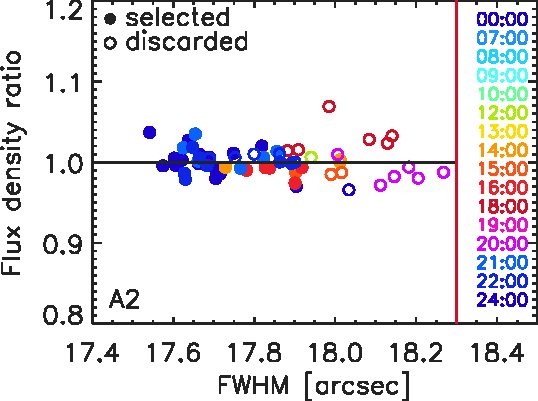
\includegraphics[clip=true, trim={0.7cm, -0.3cm, -0.25cm, 0}, width=0.465\linewidth]{Figures/plot_flux_density_ratio_fwhm_uranus_corrected_skydip_photocorr_demo_narrow_a2.pdf}
    % corr. sky. photocorr pointing
    \begin{overpic}[clip=true, trim={0, -0.3cm, -0.3cm, 0},width=0.525\linewidth]{Figures/plot_flux_density_ratio_fwhm_uranus_corrected_skydip_photocorr_pointing_narrow_1mm.pdf}
      \put(18,25){\footnotesize PC-point}
    \end{overpic}
    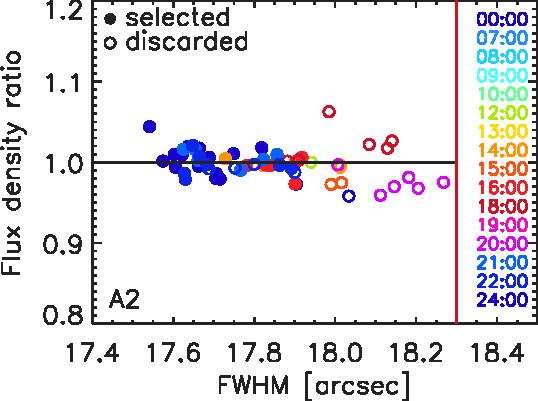
\includegraphics[clip=true, trim={0.7cm, -0.3cm, -0.25cm, 0}, width=0.465\linewidth]{Figures/plot_flux_density_ratio_fwhm_uranus_corrected_skydip_photocorr_pointing_narrow_a2.pdf}
    \vspace{-0.5cm}
    \caption[Uranus flux density stability against FWHM]{
      \small{Uranus flux density ratio vs beam size for calibration
  with photometric correction. The ratio of 
      Uranus measured flux densities to expectations as a function of the
      measured 2D Gaussian beam FWHM is shown for the $1$-mm array
      combination (left column) and for array 2 (right column) after absolute
      calibration using (\emph{first row}) the {\tt PC-demo} and (\emph{second
        row}) the {\tt PC-point} photometric corrections. These plots
      include all Uranus scans acquired during N2R9, N2R12 and N2R14
      campaigns and whose beam FWHMs are below the threshold indicated
      by the vertical red lines, (open circles), as
      well as the scans that met the baseline scan selection criteria (filled
      circles).}}
\label{fig:calib_uranus_vs_fwhm_photocorr}
\end{center}
\end{figure}

\subsubsection{Absolute calibration with a photometric correction}

We perform the absolute calibration by i) implementing the practical
method described in Sect.~\ref{se:practical_calib}, ii) correcting the
atmospheric attenuation using the {\tt corrected skydip} opacity
estimates, and iii) using the photometric correction of
Sect.~\ref{se:photometric_correction_method}.

Using the photometric correction alleviates the need of
performing a scan selection based on the observation time. However,
the scans from which the absolute calibration is derived, are selected
on the FWHM estimate using the same criteria as for the baseline
calibration, that are FWHM thresholds of $12.5''$ at $1\, \rm{mm}$ and $18''$ at
$2\, \rm{mm}$. Thus, only the scans that are moderately affected by the beam
effect are included in the absolute calibration in order not to
include twice the photometric correction uncertainties in the error
budget (once for the absolute calibration and once for the photometry).

Figure~\ref{fig:calib_uranus_vs_fwhm_photocorr} presents the Uranus
measured-to-predicted flux density ratio as a function of the beam FWHM
after the photometric correction with the {\tt PC-demo} and
{\tt PC-point} methods. The flux
density is stable against the beam FWHM within uncertainties for both
wavelengths.

% ALL METHOD RESULTS 
\begin{table}[!htbp]
\caption[Comparison of calibration results using five methods]{Comparison of absolute calibration results using five methods}
\label{tab:Abs_calibration_results_all}
\centering
\begin{tabular}{clrrrrr}
  \hline\hline
  \noalign{\smallskip}
%  \multicolumn{2}{c}{}  &  \multicolumn{5}{|c|}{Methods} \\\cline{3-7}
  \multicolumn{2}{c}{}  &  baseline  & TM\tablefootmark{a}  &  SD\tablefootmark{b} & PC-d\tablefootmark{c} & PC-p\tablefootmark{d}  \\
  \noalign{\smallskip}
  \hline\hline
   \multicolumn{2}{c}{$\#$ scans} & 26    &       26  &    26    &    38           &    38 \\ 
  \hline
  \noalign{\smallskip}
%  Factor &  A1          &   1.00  &  0.97   &  1.13    &   1.01    &   1.02  \\
%         &  A3          &   1.00  &  0.97   &  1.02    &   1.01    &   1.00  \\
   Ratio  &  1mm         &   1.00  &  0.95   &  1.06    &   1.01    &   1.01  \\
          &  2mm         &   1.00  &  0.94   &  0.99    &   1.01    &   1.01  \\
  \hline
  \noalign{\smallskip}
%  RMS  &  A1            &  3.2    &   4.2   &   3.4    &    3.5    &   3.0 \\
%  $[\%]$     &  A3      &  3.6    &   4.3   &   3.3    &    3.5    &   3.0 \\
   RMS    &  1mm           &  3.3    &   4.5   &   3.3    &    3.1    &   2.6 \\
   $[\%]$ &  2mm           &  1.6    &   2.6   &   1.5    &    1.5    &   1.5 \\
\hline
\end{tabular}
\tablefoot{ Results based on 
    \tablefoottext{a}{the {\tt Taumeter} opacity correction}
    \tablefoottext{b}{the {\tt Skydip} opacity correction}
    \tablefoottext{c}{the {\tt PC-demo} photometry correction}
    \tablefoottext{d}{the {\tt PC-point} photometry correction}
    }
\end{table}

We further quantify the
difference between all the calibration methods that have been tested
in evaluating i) the average absolute calibration factor
with respect to the baseline calibration factor and
ii) the rms dispersion of the measured-to-modeled flux ratios. These
quantities are gathered in Table~\ref{tab:Abs_calibration_results_all}
in the rows labeled 'Ratio' and 'RMS' respectively. 

We find that, resorting to a photometric correction i) allows us to use $45\%$ more
scans for the absolute calibration, ii) has a negligible impact on
the absolute calibration factor and iii) yields a small reduction of
the flux density ratio dispersion. For the absolute calibration, the
{\tt PC-point} method performs as well as the {\tt PC-demo} one.
Photometry capability and stability when using a photometric
correction will be further tested in Sect.~\ref{se:photometry}.\\

{\bf END OF OLD SECTION 8.5}\\

%\section{Photometric correction}
%\label{se:photometric_correction_detail}
%\subsection{Photometric correction}
\label{se:photometric_correction}

The effect of the telescope-driven beam size variations, as discussed
in Sect.~\ref{se:obsdate_variations}, is mitigated by correcting the measured flux
densities using a beam-size dependent function, referred to as the
photometric correction.

% flux-dependency of sigma stable
\begin{figure}[ht!]
  \begin{center}
    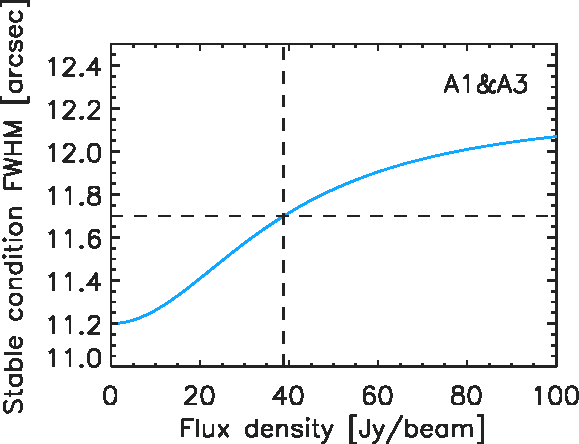
\includegraphics[clip=true, trim={0, -0.3cm, -0.3cm, 0}, width=0.45\textwidth]{Figures/atrier/Photocorr/FWHM_stable_empiric_ref_1mm.pdf}
    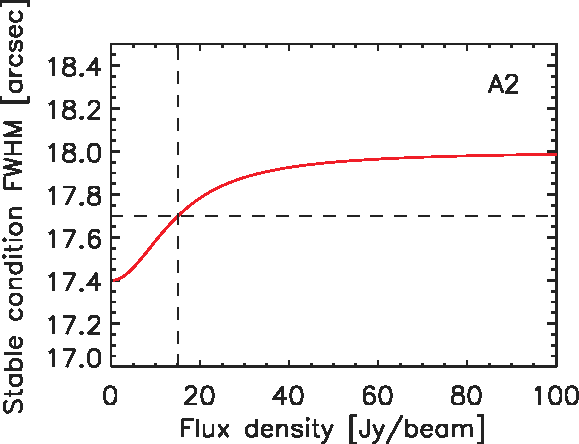
\includegraphics[clip=true, trim={0, -0.3cm, -0.3cm, 0}, width=0.45\textwidth]{Figures/atrier/Photocorr/FWHM_stable_empiric_ref_a2.pdf}
    \caption[Photometric correction pivot Gaussian
      size]{Flux-dependency of the photometric correction pivot
      Guassian size $\sigma_\star$. }
    \label{fig:sigma_stable_vs_flux}
  \end{center}
\end{figure}

In our reference photometric system, as presented in
Sect.~\ref{se:flux_density_equation} and
Sect.~\ref{ap:flux_density_equation},
the flux density is estimated by fitting an amplitude of a fixed-width
Gaussian beam:
%. Using Eqs.~\ref{eq:calfwhm0}, \ref{eq:pointsourcephot}
%and \ref{eq:pointsourcemap}, observed maps are modeled as:
%\begin{equation}
%  M(\theta, \phi) = \frac{A}{2 \pi \sigma_{0}^{2}} e^{-\frac{\theta^{2}}{2\sigma_{0}^{2}}}, 
%\end{equation}
%where $\sigma_{0}$ is the Gaussian beam size corresponding to the
%reference FWHM, which is $12.5''$ for the 1mm arrays and $18.5''$ for
%the 2mm array, as defined in Table~\ref{tab:definitions}.
\begin{equation}
  \hat{S}  = 2 \int \int M(\theta, \phi)\, e^{-\frac{\theta^{2}}{2\sigma_{0}^{2}}} \sin \theta d\theta d\phi.
  \label{eq:flux_density_estimator}
\end{equation}
The beam width $\sigma_{0}$ corresponds to the
reference FWHM, which we recall,  is $12.5''$ for the 1mm arrays and $18.5''$ for
the 2mm array, as defined in Table~\ref{tab:definitions}.

First of all, in stable observing conditions (no beam
broadening effect), the map can be modeled by a single Gaussian of
width $\sigma_\star$ corresponding basically to the main beam size:
\begin{equation}
  M(\theta, \phi) = \frac{A}{2 \pi \sigma_\star^{2}} e^{-\frac{\theta^{2}}{2\sigma_\star^{2}}}.
  \label{eq:pointsource_map}
\end{equation}
Ingesting Eq.~\ref{eq:broader_beam_map} in
Eq.~\ref{eq:flux_density_estimator}, we find that the flux density
estimator depends on the beam size as
\begin{equation}
  \hat{S}  = A \frac{2 \sigma_0^2}{(\sigma_{\star}^2 + \sigma_0^2)}.
\end{equation}
However, the map is calibrated in $FWHM_0$ beam, as described in
Sect.~\ref{se:flux_density_equation}. The absolute calibration factor,
which is evaluating as
$S_{c}(\nu_{0})/\hat{S}_{c}$, has a beam dependency that
compensates the one of the flux density for the source.

On the other hand, if the beam size varies so that the Gaussian part has a size given by
$\sigma'$, the map model rewrites  
\begin{equation}
  M(\theta, \phi) = \frac{A}{2 \pi \sigma'^{2}} e^{-\frac{\theta^{2}}{2\sigma'^{2}}},
  \label{eq:broader_beam_map}
\end{equation}
where the amplitude is the same as in the stable condition case
because the flux density is conserved when integrating over the map. 
The flux density measured using the fixed-width amplitude estimator 
\begin{equation}
  \hat{S'}  = A \frac{2 \sigma_0^2}{(\sigma'^2 + \sigma_0^2)}
\end{equation}
presents a beam-dependency which differs from the one of the primary
calibrator, and which is no longer compensated when performing the
absolute calibration.

To retrieve an unbiased flux density estimate $\hat{S}_{pc}$, the
flux density estimate $\hat{S'}$ has to be corrected as
\begin{equation}
  \hat{S}_{pc} = f(\sigma')\hat{S'},
\end{equation} 
where the photometric correction is 
\begin{equation}
  f(\sigma') = \frac{(\sigma'^2 + \sigma_0^2)}{(\sigma_\star^2+\sigma_0^2)}, 
\end{equation} 
so that $f(\sigma') = 1$ if $\sigma'=\sigma_\star$.

The pivot Gaussian size $\sigma_{\star}$, which corresponds
to the nominal size of the 2D Gaussian fit of the beam that is
measured in stable observing conditions, slightly varies with the
source flux density. Whereas it basically corresponds to the main beam
size for faint to moderately bright point source, it is slightly
larger for sources bright enought for the error beams to be well above
the noise level. In Fig.~\ref{fig:sigma_stable_vs_flux}, we give an
empirical model for the flux dependency of $\sigma_{\star}$: it
smoothly goes from $11.2''$ at 1-mm and $17.4''$ at 2-mm for
moderately bright sources to
$11.7''$ at 1-mm and $17.7''$ at 2-mm at the flux density of Uranus,
then slightly continues increasing for sources brighter than Uranus.


The effect of the \afternoon\ beam size variations, as discussed
in Sect.~\ref{se:beam_variation}, is mitigated by correcting the
measured flux densities using a beam-size dependent function, referred
to as the photometric correction.

In our reference photometric system, as presented in
Sect.~\ref{se:photometric_system}, 
the flux density is estimated by fitting to the data the amplitude of
the FWHM$_0$ Gaussian beam:
\begin{equation}
  \hat{S}  = 2 \int \int M(\theta, \phi)\, e^{-\frac{\theta^{2}}{2\sigma_{0}^{2}}} \sin \theta d\theta d\phi.
  \label{eq:flux_density_estimator}
\end{equation}
The beam width $\sigma_{0}$ corresponds to FWHM$_0$%, which we recall,
%is $12.5''$ for the $1\,\rm{mm}$ arrays and $18.5''$ for
%the $2\,\rm{mm}$ array
, as defined in Table~\ref{tab:definitions}.


First of all, in stable observing conditions (no beam
broadening effect), the observed map of a point-like source can be modeled by a single Gaussian of
width $\sigma_\star$ corresponding basically to the main beam size and
of amplitude $A_\star$:
\begin{equation}
  M(\theta, \phi) = A_\star e^{-\frac{\theta^{2}}{2\sigma_\star^{2}}}.
  \label{eq:pointsource_map}
\end{equation}
Ingesting Eq.~\ref{eq:pointsource_map} in
Eq.~\ref{eq:flux_density_estimator}, we find that the flux density
estimator depends on the beam size as
\begin{equation}
  \hat{S}  = 2\pi \sigma_{\star}^2 \, A_{\star} \, \,  \frac{2 \sigma_0^2}{(\sigma_{\star}^2 + \sigma_0^2)}.
  \label{eq:gaussian_star}
\end{equation}
However, the map is calibrated using FWHM$_0$ Gaussian beam, as described in
Sect.~\ref{se:photometric_system}. The absolute calibration factor %,
%which is evaluating as
%$S_{c}(\nu_{0})/\hat{S}_{c}$,
has a beam dependency that compensates the one of the flux density for the source.

On the other hand, if the beam size varies so that the Gaussian part has a size given by
$\sigma'$, Eq.~\ref{eq:gaussian_star} could be rewritten as 
\begin{equation}
  M(\theta, \phi) = A'\, e^{-\frac{\theta^{2}}{2\sigma'^{2}}}.
  \label{eq:broader_beam_map}
\end{equation}

The flux density measured using the reference beam amplitude estimator 
\begin{equation}
  \hat{S'}  =2\pi \sigma'^2 \, A' \, \,  \frac{2 \sigma_0^2}{(\sigma'^2 + \sigma_0^2)}
\end{equation}
presents a beam-dependency which differs from the one of the primary
calibrator, and which is no longer compensated when performing the
absolute calibration.

{\lp In addition, because the flux density is conserved when integrating over the map,
the Gaussian amplitudes verify
\begin{equation}
2\pi \sigma_{\star}^2 \, A_{\star} = 2\pi \sigma'^2 \, A'
\label{eq:gaussian_amplitude}
\end{equation}}

To retrieve an unbiased flux density estimate $\hat{S}_{\rm{pc}}$, the
flux density estimate $\hat{S'}$ has to be corrected as
\begin{equation}
  \hat{S}_{\rm{pc}} = f(\sigma') \, \hat{S'},
\end{equation} 
where the photometric correction is 
\begin{equation}
  f(\sigma') = \frac{(\sigma'^2 + \sigma_0^2)}{(\sigma_\star^2+\sigma_0^2)}, 
\end{equation} 
so that $f(\sigma') = 1$ if $\sigma'=\sigma_\star$.

% flux-dependency of sigma stable
\begin{figure}[ht!]
  \begin{center}
    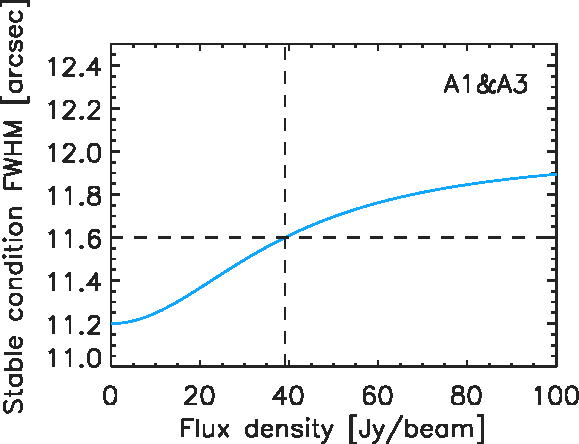
\includegraphics[clip=true, trim={0, -0.3cm, -0.3cm, 0}, width=0.49\linewidth]{Figures/FWHM_stable_empiric_ref_1mm.pdf}
    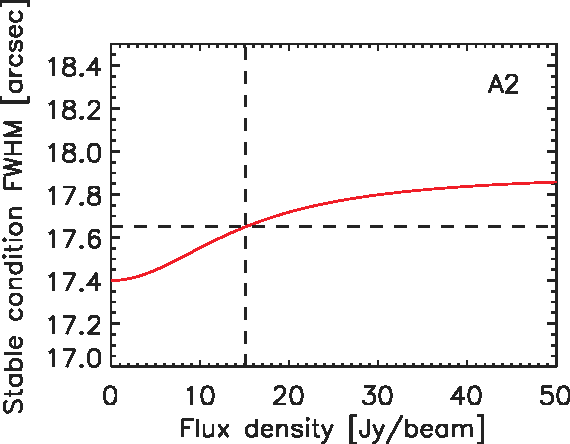
\includegraphics[clip=true, trim={0, -0.3cm, -0.3cm, 0}, width=0.49\linewidth]{Figures/FWHM_stable_empiric_ref_a2.pdf}
    \caption[Photometric correction pivot Gaussian
      size]{Flux-dependency of the pivot size $\sigma_\star$ of the
      Gaussian beam used for the photometric correction. %This is measured as the 2D
      %Gaussian fit of the map observed in stable conditions.
      The vertical dashed lines correspond to Uranus flux densities in
      the two bands, and the horizontal dashed lines are the FWHMs
    corresponding to the measured $\sigma_\star$ towards Uranus.}
    \label{fig:sigma_stable_vs_flux}
  \end{center}
\end{figure}

As discussed in Sect.~\ref{se:beam_variation}, the beam size is
monitored by fitting a 2D Gaussian of freely varying FWHM.
%In practice,
%the pivot Gaussian size $\sigma_{\star}$ thus corresponds
%to the nominal size of the 2D Gaussian fit of the beam that is
%measured in stable observing conditions.
We find the Gaussian size $\sigma_{\star}$ slightly varies with the
source flux density. Whereas it basically corresponds to the main beam
size for faint to moderately bright point source, it is slightly
larger for bright sources. The simple 2D Gaussian fit
accomodates with the more complex beam pattern features that are well
above the noise level (see Sect.~\ref{se:fullbeam}) in tha case of
bright sources.
%bright enough for the side lobes to be well above the noise level.
%The variation of $\sigma_{\star}$ can be seen as a
%correction for fitting the complex beam pattern, as presented in
%Sect.~\ref{se:fullbeam}, with a single 2D Gaussian of freely varying
%size.

In Fig.~\ref{fig:sigma_stable_vs_flux}, we give an
empirical model for the flux dependency of the FWHM derived from
$\sigma_{\star}$: it
smoothly goes from $11.2''$ at $1\,\rm{mm}$ and $17.4''$ at $2\,\rm{mm}$ for
faint sources to $11.6''$ at $1\,\rm{mm}$ and $17.65''$ at
$2\,\rm{mm}$ at the flux density of Uranus,
then slightly continues increasing for sources brighter than Uranus.
